\documentclass{standalone}
\usepackage{tikz}
\usetikzlibrary{patterns, positioning}
\usepackage[sfdefault]{ClearSans} %% option 'sfdefault' activates Clear Sans as the default text font
\usepackage[T1]{fontenc}

\begin{document}
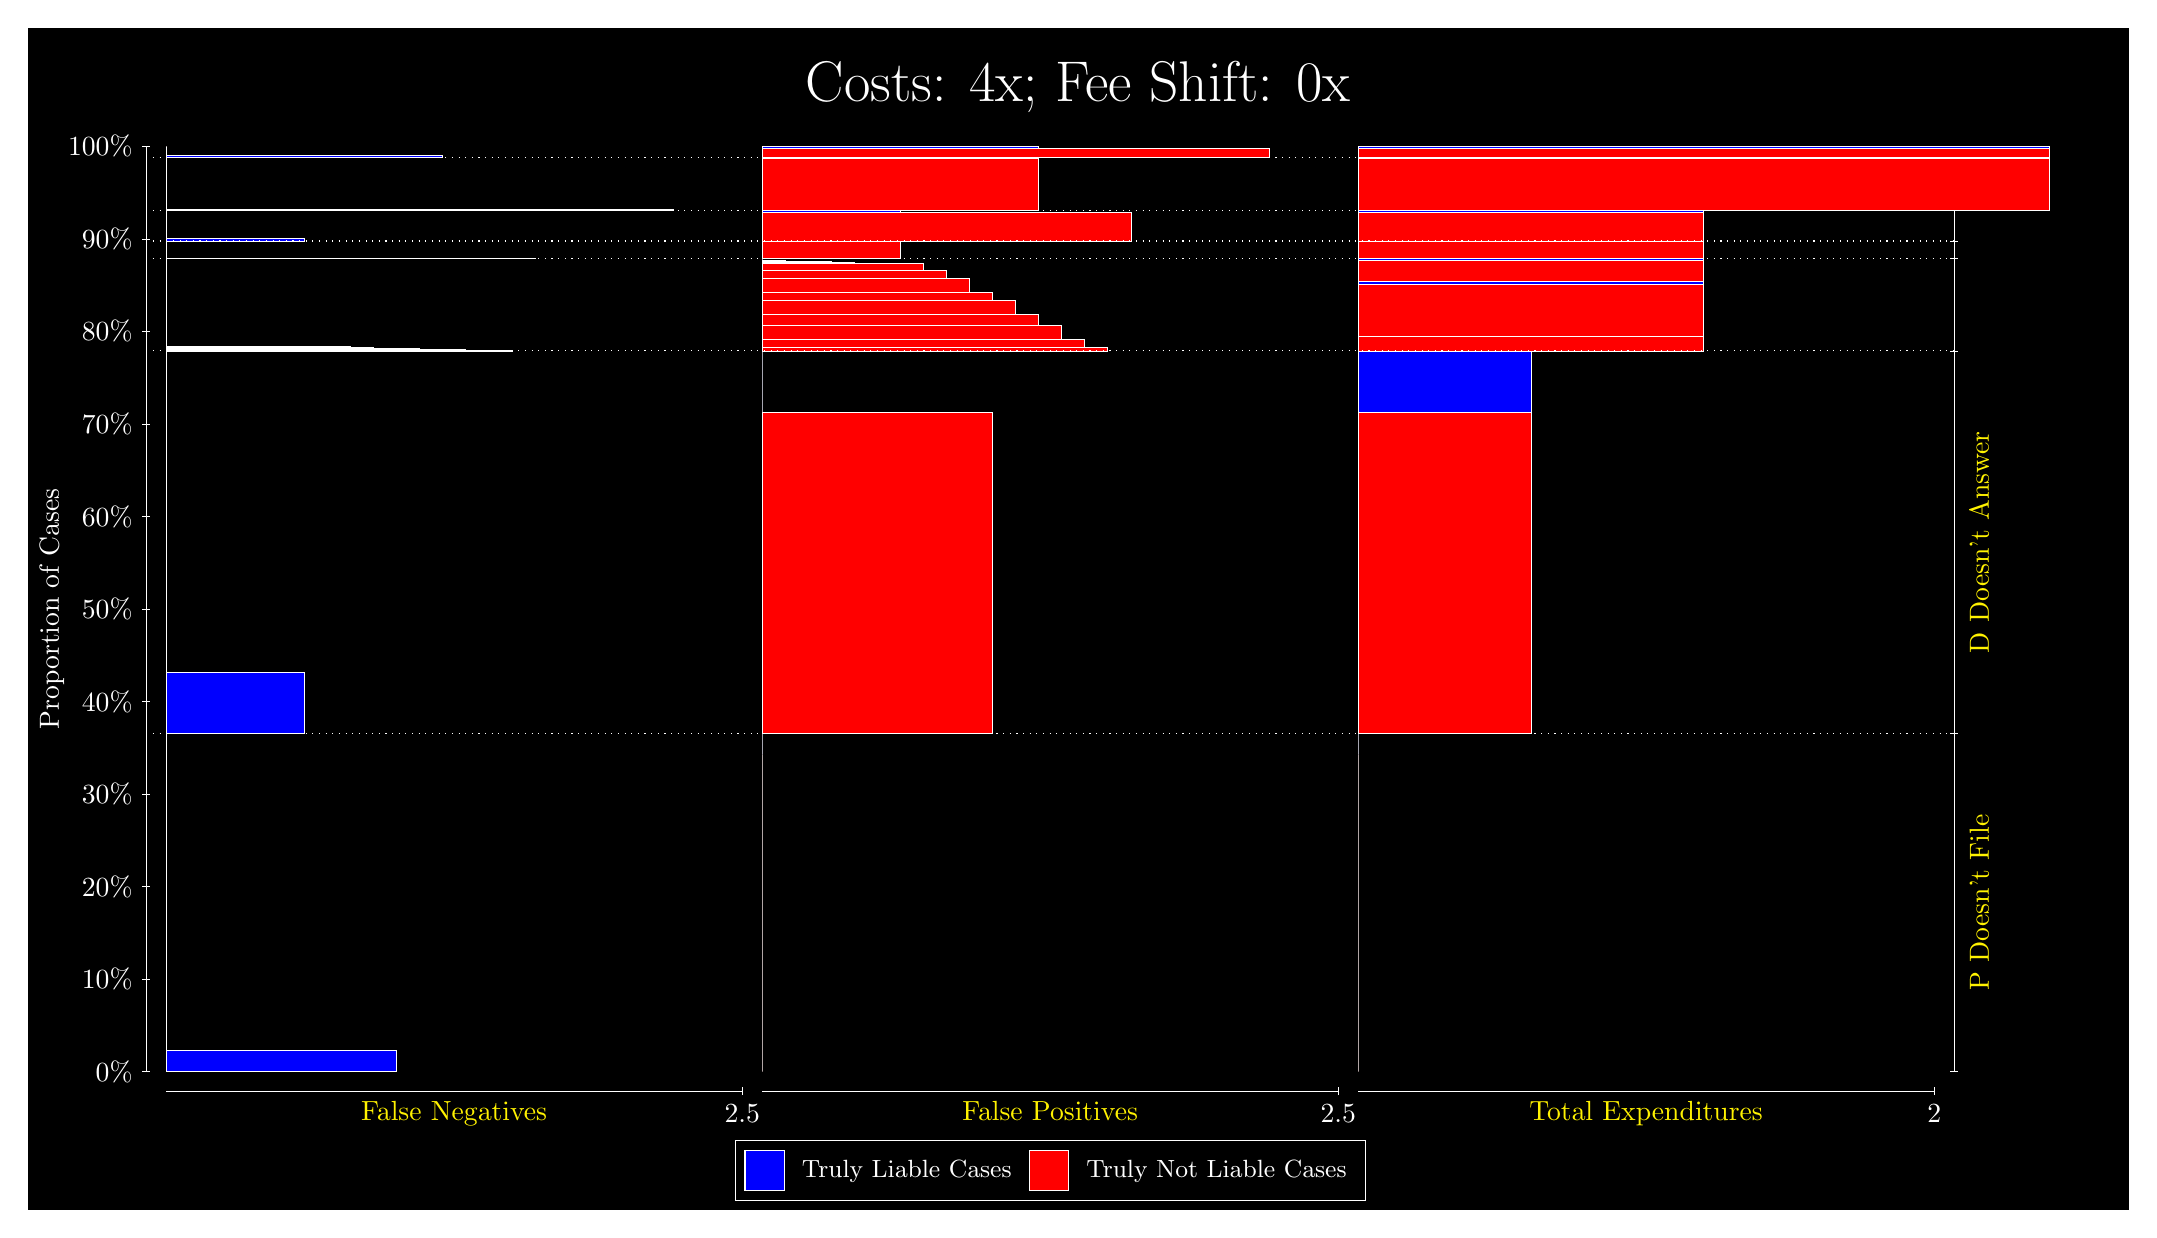
\begin{tikzpicture}
\draw[fill=black] (0,0) rectangle (26.667,15);
\draw[text=white] (0,13.5) rectangle (26.667,15) node[midway] {\huge Costs: 4x; Fee Shift: 0x};
\draw[white, very thin] (1.5,1.75) -- (1.5,13.5);
\node[rotate=90, text=white, anchor=center] at (0.3, 7.625) {Proportion of Cases};
\draw[white, very thin] (1.45,1.75) -- (1.55,1.75);
\node[text=white, anchor=east] at (1.45, 1.75) {0\%};
\draw[white, very thin] (1.45,2.925) -- (1.55,2.925);
\node[text=white, anchor=east] at (1.45, 2.925) {10\%};
\draw[white, very thin] (1.45,4.1) -- (1.55,4.1);
\node[text=white, anchor=east] at (1.45, 4.1) {20\%};
\draw[white, very thin] (1.45,5.275) -- (1.55,5.275);
\node[text=white, anchor=east] at (1.45, 5.275) {30\%};
\draw[white, very thin] (1.45,6.45) -- (1.55,6.45);
\node[text=white, anchor=east] at (1.45, 6.45) {40\%};
\draw[white, very thin] (1.45,7.625) -- (1.55,7.625);
\node[text=white, anchor=east] at (1.45, 7.625) {50\%};
\draw[white, very thin] (1.45,8.8) -- (1.55,8.8);
\node[text=white, anchor=east] at (1.45, 8.8) {60\%};
\draw[white, very thin] (1.45,9.975) -- (1.55,9.975);
\node[text=white, anchor=east] at (1.45, 9.975) {70\%};
\draw[white, very thin] (1.45,11.15) -- (1.55,11.15);
\node[text=white, anchor=east] at (1.45, 11.15) {80\%};
\draw[white, very thin] (1.45,12.325) -- (1.55,12.325);
\node[text=white, anchor=east] at (1.45, 12.325) {90\%};
\draw[white, very thin] (1.45,13.5) -- (1.55,13.5);
\node[text=white, anchor=east] at (1.45, 13.5) {100\%};

\draw[white, very thin] (24.457,1.75) -- (24.457,13.5);
\draw[white, very thin] (24.407,1.75) -- (24.507,1.75);
\node[anchor=west] at (24.407, 1.75) {};
\draw[white, very thin] (24.407,6.0439) -- (24.507,6.0439);
\node[anchor=west] at (24.407, 6.0439) {};
\draw[white, very thin] (24.407,10.902) -- (24.507,10.902);
\node[anchor=west] at (24.407, 10.902) {};
\draw[white, very thin] (24.407,12.074) -- (24.507,12.074);
\node[anchor=west] at (24.407, 12.074) {};
\draw[white, very thin] (24.407,12.298) -- (24.507,12.298);
\node[anchor=west] at (24.407, 12.298) {};
\draw[white, very thin] (24.407,12.689) -- (24.507,12.689);
\node[anchor=west] at (24.407, 12.689) {};
\draw[white, very thin] (24.407,13.355) -- (24.507,13.355);
\node[anchor=west] at (24.407, 13.355) {};
\draw[white, very thin] (24.407,13.5) -- (24.507,13.5);
\node[anchor=west] at (24.407, 13.5) {};

\draw[white, very thin, fill=blue] (1.75,1.75) rectangle (4.6775,2.0148);
\draw[white, very thin, fill=red] (1.75,2.0148) rectangle (1.75,6.0439);
\draw[white, very thin, fill=blue] (1.75,6.0439) rectangle (3.5065,6.8205);
\draw[white, very thin, fill=red] (1.75,6.8205) rectangle (1.75,10.902);
\draw[white, very thin, fill=blue] (1.75,10.902) rectangle (6.1413,10.907);
\draw[white, very thin, fill=blue] (1.75,10.907) rectangle (5.8486,10.912);
\draw[white, very thin, fill=blue] (1.75,10.912) rectangle (5.5558,10.919);
\draw[white, very thin, fill=blue] (1.75,10.919) rectangle (5.2631,10.924);
\draw[white, very thin, fill=blue] (1.75,10.924) rectangle (4.9703,10.932);
\draw[white, very thin, fill=blue] (1.75,10.932) rectangle (4.6775,10.937);
\draw[white, very thin, fill=blue] (1.75,10.937) rectangle (4.3848,10.948);
\draw[white, very thin, fill=blue] (1.75,10.948) rectangle (4.092,10.955);
\draw[white, very thin, fill=blue] (1.75,10.955) rectangle (3.7993,10.961);
\draw[white, very thin, fill=red] (1.75,10.961) rectangle (1.75,12.074);
\draw[white, very thin, fill=blue] (1.75,12.074) rectangle (6.4341,12.082);
\draw[white, very thin, fill=red] (1.75,12.082) rectangle (1.75,12.298);
\draw[white, very thin, fill=blue] (1.75,12.298) rectangle (3.5065,12.327);
\draw[white, very thin, fill=red] (1.75,12.327) rectangle (1.75,12.689);
\draw[white, very thin, fill=blue] (1.75,12.689) rectangle (8.1906,12.703);
\draw[white, very thin, fill=red] (1.75,12.703) rectangle (1.75,13.355);
\draw[white, very thin, fill=blue] (1.75,13.355) rectangle (5.2631,13.38);
\draw[white, very thin, fill=red] (1.75,13.38) rectangle (1.75,13.5);
\draw[white, very thin, fill=red] (9.3189,1.75) rectangle (9.3189,5.779);
\draw[white, very thin, fill=blue] (9.3189,5.779) rectangle (9.3189,6.0439);
\draw[white, very thin, fill=red] (9.3189,6.0439) rectangle (12.246,10.125);
\draw[white, very thin, fill=blue] (9.3189,10.125) rectangle (9.3189,10.902);
\draw[white, very thin, fill=red] (9.3189,10.902) rectangle (13.71,10.948);
\draw[white, very thin, fill=red] (9.3189,10.948) rectangle (13.417,11.044);
\draw[white, very thin, fill=red] (9.3189,11.044) rectangle (13.125,11.223);
\draw[white, very thin, fill=red] (9.3189,11.223) rectangle (12.832,11.363);
\draw[white, very thin, fill=red] (9.3189,11.363) rectangle (12.539,11.544);
\draw[white, very thin, fill=red] (9.3189,11.544) rectangle (12.246,11.643);
\draw[white, very thin, fill=red] (9.3189,11.643) rectangle (11.954,11.829);
\draw[white, very thin, fill=red] (9.3189,11.829) rectangle (11.661,11.929);
\draw[white, very thin, fill=red] (9.3189,11.929) rectangle (11.368,12.016);
\draw[white, very thin, fill=blue] (9.3189,12.016) rectangle (10.783,12.021);
\draw[white, very thin, fill=blue] (9.3189,12.021) rectangle (10.49,12.029);
\draw[white, very thin, fill=blue] (9.3189,12.029) rectangle (10.197,12.039);
\draw[white, very thin, fill=blue] (9.3189,12.039) rectangle (9.9044,12.044);
\draw[white, very thin, fill=blue] (9.3189,12.044) rectangle (9.6116,12.052);
\draw[white, very thin, fill=blue] (9.3189,12.052) rectangle (9.3189,12.074);
\draw[white, very thin, fill=red] (9.3189,12.074) rectangle (11.075,12.291);
\draw[white, very thin, fill=blue] (9.3189,12.291) rectangle (9.3189,12.298);
\draw[white, very thin, fill=red] (9.3189,12.298) rectangle (14.003,12.66);
\draw[white, very thin, fill=blue] (9.3189,12.66) rectangle (11.075,12.689);
\draw[white, very thin, fill=red] (9.3189,12.689) rectangle (12.832,13.342);
\draw[white, very thin, fill=blue] (9.3189,13.342) rectangle (9.9044,13.355);
\draw[white, very thin, fill=red] (9.3189,13.355) rectangle (15.759,13.475);
\draw[white, very thin, fill=blue] (9.3189,13.475) rectangle (12.832,13.5);
\draw[white, very thin, fill=red] (16.888,1.75) rectangle (16.888,5.779);
\draw[white, very thin, fill=blue] (16.888,5.779) rectangle (16.888,6.0439);
\draw[white, very thin, fill=red] (16.888,6.0439) rectangle (19.083,10.125);
\draw[white, very thin, fill=blue] (16.888,10.125) rectangle (19.083,10.902);
\draw[white, very thin, fill=red] (16.888,10.902) rectangle (21.279,11.083);
\draw[white, very thin, fill=blue] (16.888,11.083) rectangle (21.279,11.091);
\draw[white, very thin, fill=red] (16.888,11.091) rectangle (21.279,11.748);
\draw[white, very thin, fill=blue] (16.888,11.748) rectangle (21.279,11.781);
\draw[white, very thin, fill=red] (16.888,11.781) rectangle (21.279,12.057);
\draw[white, very thin, fill=blue] (16.888,12.057) rectangle (21.279,12.074);
\draw[white, very thin, fill=red] (16.888,12.074) rectangle (21.279,12.291);
\draw[white, very thin, fill=blue] (16.888,12.291) rectangle (21.279,12.298);
\draw[white, very thin, fill=red] (16.888,12.298) rectangle (21.279,12.66);
\draw[white, very thin, fill=blue] (16.888,12.66) rectangle (21.279,12.689);
\draw[white, very thin, fill=red] (16.888,12.689) rectangle (25.67,13.342);
\draw[white, very thin, fill=blue] (16.888,13.342) rectangle (25.67,13.355);
\draw[white, very thin, fill=red] (16.888,13.355) rectangle (25.67,13.475);
\draw[white, very thin, fill=blue] (16.888,13.475) rectangle (25.67,13.5);
\draw[white, dotted] (1.5,6.0439) -- (24.457,6.0439);
\draw[white, dotted] (1.5,10.902) -- (24.457,10.902);
\draw[white, dotted] (1.5,12.074) -- (24.457,12.074);
\draw[white, dotted] (1.5,12.298) -- (24.457,12.298);
\draw[white, dotted] (1.5,12.689) -- (24.457,12.689);
\draw[white, dotted] (1.5,13.355) -- (24.457,13.355);
\draw[white, very thin] (1.75,1.5) -- (9.0689,1.5);
\node[text=yellow, anchor=north] at (5.4094, 1.5) {False Negatives};
\draw[white, very thin] (9.0689,1.45) -- (9.0689,1.55);
\node[text=white, anchor=north] at (9.0689, 1.45) {2.5};

\draw[white, very thin] (9.3189,1.5) -- (16.638,1.5);
\node[text=yellow, anchor=north] at (12.978, 1.5) {False Positives};
\draw[white, very thin] (16.638,1.45) -- (16.638,1.55);
\node[text=white, anchor=north] at (16.638, 1.45) {2.5};

\draw[white, very thin] (16.888,1.5) -- (24.207,1.5);
\node[text=yellow, anchor=north] at (20.547, 1.5) {Total Expenditures};
\draw[white, very thin] (24.207,1.45) -- (24.207,1.55);
\node[text=white, anchor=north] at (24.207, 1.45) {2};

\node[text=yellow, centered, rotate=90] at (24.777, 3.8969) {P Doesn't File};
\node[text=yellow, centered, rotate=90] at (24.777, 8.473) {D Doesn't Answer};






\draw (12.978300999999998,1.5) node[draw=none] (baseCoordinate) {};
\begin{scope}[align=center]
        \matrix[scale=0.5, draw=white, below=0.5cm of baseCoordinate, nodes={draw}, column sep=0.1cm]{
            \node[rectangle, draw, minimum width=0.5cm, minimum height=0.5cm, fill=blue] {}; &
            \node[draw=none, font=\small, text=white] (B) {Truly Liable Cases}; &
            \node[rectangle, draw, minimum width=0.5cm, minimum height=0.5cm, fill=red] {}; &
            \node[draw=none, font=\small, text=white] (B) {Truly Not Liable Cases}; \\
            };
\end{scope}

\end{tikzpicture}
\end{document}